\documentclass[11pt]{article}

\usepackage{amsmath,amssymb,amsfonts}
\usepackage{geometry}
\geometry{margin=1in}
\usepackage{hyperref}
\usepackage{graphicx}
\usepackage{booktabs}
\usepackage{float} % for [H]: keeps figures/tables where they're placed in the source instead of drifting to the end
\graphicspath{{figures/}}

\title{Snowball Contamination of Compact, Red Source Selections in JWST NIRCam Imaging:\\
A Case Study Motivated by the ``Little Red Dot'' Population}

\author{Paul Jarvis \\
Independent Researcher, UK \\
\texttt{mrpaulwjarvis@gmail.com} \\
ORCID: \href{https://orcid.org/0009-0009-8933-857X}{0009-0009-8933-857X}}

\date{August 13, 2026}

\begin{document}

\maketitle

\begin{abstract}
JWST's ``Little Red Dots'' (LRDs), compact, point-source-like, red-continuum
sources found in large numbers in deep NIRCam surveys, are selected on a basic
photometric signature: compact morphology plus a smooth, red spectral shape. We
test how much of that signature, in NIRCam mosaics this project has already
processed for an unrelated dropout-galaxy search, survives contact with the raw
detector data. A crude proxy for LRD-like selection, built from columns this
project's existing pipeline already produces, flags 25 candidates across four
independently-searched fields (SMACS J0723.3$-$7327, A2744/UNCOVER, GOODS-N,
JADES/GOODS-S). Of the 22 candidates in fields that had not previously received
full visual vetting, roughly 70-75\% show a visual signature consistent with a
detector artifact or a blended neighbor rather than a clean point source. We take
this further than eyeballing: installing \texttt{snowblind}, the field-standard
tool for exactly this problem, and running the real \texttt{Detector1Pipeline} on
raw exposures for every flagged candidate's tile, we confirm 7 of 22 (32\%) are
genuine NIRCam ``snowball'' cosmic-ray artifacts, using a persistence criterion a
stochastic detector event cannot satisfy but a real astrophysical source
routinely does: transient saturation present in some, but not all, exposures that
independently cover the same sky position. The one field where the proxy
selection came back clean (SMACS, 3 of 3) is also the only field whose candidates
had already been through this project's full multi-round vetting before this
study began; the determining factor is vetting status, not field identity. The
originally-suspected contaminant motivating this study, a NIRCam module A/B
background offset previously found and corrected in this project's own dropout
search, turns out not to be the dominant mechanism here; snowball contamination
of low-exposure-redundancy tiles is. This is a known phenomenon in the JWST
literature, not a new discovery, but this project's own measurement is an
independent, if crude, quantification of a gap the field's own reduction papers
acknowledge leaving open. We extend the test to a fifth, independent field: the
first public Deep-tier data release of NEXUS, a JWST Treasury survey whose
two-point-dither imaging strategy the survey's own documentation already flags
as a known artifact risk. Applying the identical raw-DQ persistence method to an
independently-built 18-candidate proxy sample from this new survey confirms 2 of
18 (11\%) as real, single-epoch transient artifacts, extending rather than merely
repeating this paper's original finding to a brand-new 2026 data release.
\end{abstract}

\section{Introduction}

``Little Red Dots'' are a population of compact, red, point-source-like objects
discovered in large numbers by JWST NIRCam deep and cluster-field surveys,
essentially unknown before JWST began operating. Their nature is actively
contested. High-resolution spectroscopy of the reddest, most extreme examples
has been interpreted as young supermassive black holes embedded in dense,
ionized-gas cocoons, with electron scattering rather than orbital motion
broadening their emission lines \cite{Rusakov2026}. A separate, contemporaneous
review pushes back on treating the AGN-cocoon picture as settled, noting that a
dusty star-forming origin cannot yet be excluded for the population as a whole
\cite{InayoshiHo2025}.

This paper does not attempt to adjudicate that debate. It asks a narrower,
selection-level question, motivated by a systematic this project had already
found and corrected in an unrelated context: a real NIRCam module A/B background
offset that flipped the blue/red classification of two high-redshift dropout
candidates in this project's own SMACS J0723.3$-$7327 and JADES/GOODS-S search
\cite{Jarvis2026a}. LRDs are selected on exactly the kind of multi-band color and
compactness signature that a background systematic of that kind could plausibly
distort. The question tested here: how much of the LRD-like color/compactness
signature, in NIRCam mosaics this project has already processed, survives
scrutiny once the underlying detector data is actually checked?

A short literature check before committing time to this (four searches, not a
full review) found the specific question, whether this project's own
already-known module A/B offset affects LRD-selected sources, genuinely
untouched, while confirming the broader category (selection-systematics scrutiny
of LRD samples) is an active area generally, not virgin territory
\cite{Hviding2025,Langeroodi2023}.

\section{Selection and Fields}

We reuse, without modification, the NIRCam mosaics, background-correction code,
and candidate catalogs already produced by this project's dropout-search pipeline
\cite{Jarvis2026a} across four independently-searched fields: SMACS
J0723.3$-$7327, A2744/UNCOVER, GOODS-N, and JADES/GOODS-S. All catalogs used are
the current-best generation of background correction available for each field
(source-masked local background, the third and most recent generation of the fix
described in \cite{Jarvis2026a}), so any contamination found here is not simply a
restatement of the already-corrected background systematic.

A crude proxy for LRD-like selection was built from columns the existing pipeline
already produces: not a real LRD selection (no rest-UV slope fit, no formal
V-shape fit, no morphology beyond a concentration index):
\begin{itemize}
    \item concentration index in $[0.65, 1.00]$ (compact, and within the
    pipeline's own physically valid range; values above 1.00 are already an
    established artifact signature in this project's data, not a real compact
    source);
    \item mid-band break-shape classification equal to
    \texttt{smooth\_dusty\_interloper\_like} (a gradual red continuum, closer to
    an LRD's V-shape than to a sharp Lyman break).
\end{itemize}

Applied to the current-best candidate catalog for each field, this flags 25
candidates: 3 in SMACS, 8 in A2744, 8 in GOODS-N, 6 in JADES/GOODS-S
(Table~\ref{tab:proxy_counts}). SMACS's 3 candidates had already been through
this project's full multi-round vetting (visual inspection, SIMBAD/Gaia/VizieR
crossmatch, local-background recheck, and in one case archival grism extraction)
in earlier, unrelated work and are treated here as a baseline rather than
re-tested; the remaining 22, across the other three fields, had not received
equivalent scrutiny before this study.

\begin{table}[H]
\centering
\caption{LRD-like-proxy candidates flagged per field.}
\label{tab:proxy_counts}
\begin{tabular}{lc}
\toprule
Field & Proxy-flagged candidates \\
\midrule
SMACS J0723.3$-$7327 & 3 \\
A2744/UNCOVER         & 8 \\
GOODS-N                & 8 \\
JADES/GOODS-S           & 6 \\
\midrule
Total                   & 25 \\
\bottomrule
\end{tabular}
\end{table}

\section{Round 1: Visual Vetting}

Each of the 22 non-SMACS candidates' cutouts (generated fresh for A2744 and
GOODS-N, which had never received any visual vetting at all prior to this study;
already available for JADES) was eyeballed against two failure signatures this
project had already characterized in earlier, unrelated work: hard-edged, blocky
pixels with no smooth PSF falloff (a detector-artifact signature), and an
aperture sitting on the wing of a bright, extended neighbor (a blend-contamination
signature). This is stated up front as eyeball pattern-matching, not a validated
statistic; this project independently attempted and abandoned five quantitative
versions of similar artifact-calling in earlier work, none of which passed
population-level validation.

\begin{table}[H]
\centering
\caption{Round 1 visual vetting results, non-SMACS fields.}
\label{tab:round1}
\begin{tabular}{lccc}
\toprule
Field & Looks clean & Blocky-artifact-like & Blend/bright-star-like \\
\midrule
JADES (6)    & 2 & 2 & 2 \\
A2744 (8)    & 2 & 3 & 3 \\
GOODS-N (8)  & 2 & 4 & 2 \\
\bottomrule
\end{tabular}
\end{table}

Roughly 70-75\% of the flagged candidates in each field show a suggestive
contamination signature under this pass. The clean-fraction contrast with SMACS
(3 of 3 clean under the same proxy) is the first indication that field identity
is not the operative variable; vetting history is.

\section{Round 2: Raw-Pipeline Verification}

Visual pattern-matching alone is not a validated statistic in this project's own
prior experience, so we escalated to the field's actual standard tool for this
exact problem: \texttt{snowblind} \cite{Davies2024snowblind}, used by major
LRD-focused surveys (RUBIES, PANORAMIC) specifically because LRDs' point-like
appearance in the reddest NIRCam bands makes them easy to confuse with cosmic-ray
snowball events \cite{Hviding2025}.

For each of the 12 tiles hosting the 22 non-SMACS candidates, we downloaded the
raw \texttt{\_uncal.fits} exposures (both \texttt{nrcalong}/\texttt{nrcblong}
modules) and ran the real \texttt{Detector1Pipeline} (dark current subtraction,
jump detection with \texttt{snowblind}'s \texttt{SnowblindStep} post-hook, ramp
fitting) to completion, rather than relying on the Stage-3 resampled mosaic. For
each candidate, we identified which raw exposures actually cover its sky
position, using a real distortion-corrected WCS solution (\texttt{AssignWcsStep})
rather than the coarse pointing-only WCS Detector1 carries by default.

The decisive test applies a persistence criterion a stochastic detector event
cannot satisfy: a genuinely bright astrophysical source saturates in every
exposure that covers its position, since flux does not disappear between two
independent looks at the same sky position taken minutes apart in the same visit;
a cosmic-ray/snowball hit is stochastic per-exposure and will not. We flag a
candidate as artifact-consistent when \texttt{SATURATED} (DQ bit 2) flags are
present in some, but not all, of its covering exposures.

\subsection{Case study: GOODS-N candidate 973}

The single most extreme candidate in the proxy sample (11238$\sigma$ in the
original detection) provides the cleanest illustration of the method. Only 2 of
12 downloaded exposures for its tile actually cover its sky position on-detector.
Exposure \texttt{00005} shows an 8$\times$6-pixel \texttt{SATURATED} footprint
sitting exactly on the candidate's position, a real, spatially extended
saturation event, not a single stray pixel, while a same-exposure control region
200 pixels away has zero saturated pixels in an identically sized box. Exposure
\texttt{00006}, covering the same sky position from a $\sim$10-pixel dithered
offset, has zero saturated pixels at the candidate's position. Saturation present
in exactly one of two independent looks at the same sky position, taken minutes
apart in the same visit, is not a signature a real source can produce
(Fig.~\ref{fig:cutout_973}).

\begin{figure}[H]
\centering
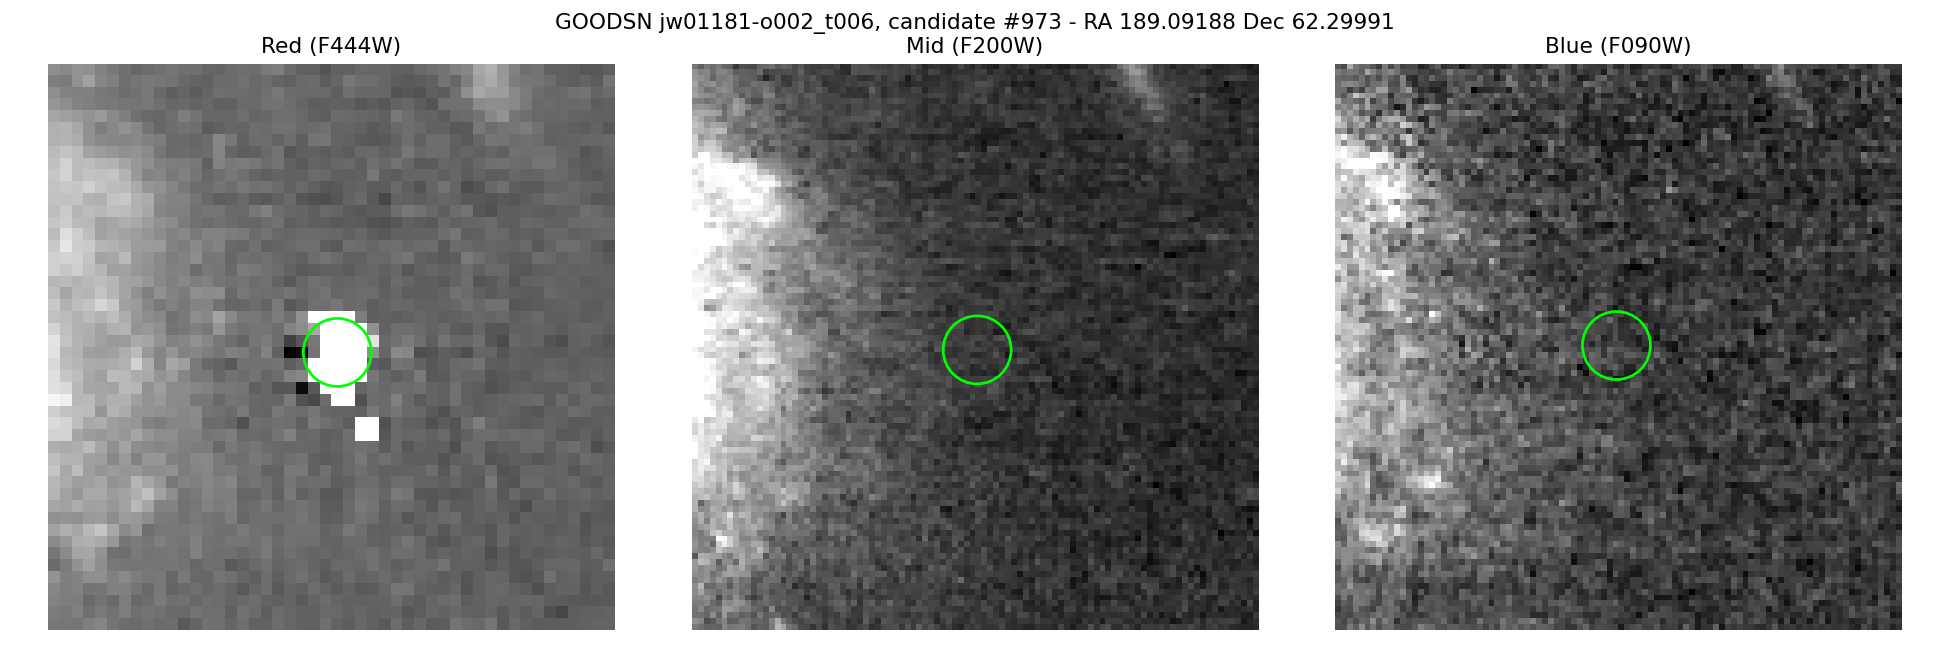
\includegraphics[width=\linewidth]{cutout_973.png}
\caption{GOODS-N candidate \#973 (11238$\sigma$ in the original LRD-like-proxy
detection), the decisive case study. Raw-exposure DQ flags confirm this is a
single-epoch snowball/cosmic-ray artifact, not a real source (Sec.~4.1).}
\label{fig:cutout_973}
\end{figure}

\subsection{Full sample results}

Applying the same criterion to all 22 candidates (Table~\ref{tab:round2}):

\begin{table}[H]
\centering
\caption{Round 2 raw-pipeline verification, all 22 non-SMACS candidates.}
\label{tab:round2}
\begin{tabular}{lc}
\toprule
Outcome & Candidates \\
\midrule
Confirmed artifact-consistent (partial-exposure saturation) & 7 \\
Plausibly real (modest, partial saturation, independently corroborated) & 3 \\
Confirmed clean by raw pipeline (zero saturation, all covering exposures) & 7 \\
Visual pass only, not raw-pipeline-tested (see caveat below) & 1 \\
Inconclusive (candidate position off-detector in all downloaded exposures) & 4 \\
\midrule
Total & 22 \\
\bottomrule
\end{tabular}
\end{table}

\begin{figure}[H]
\centering
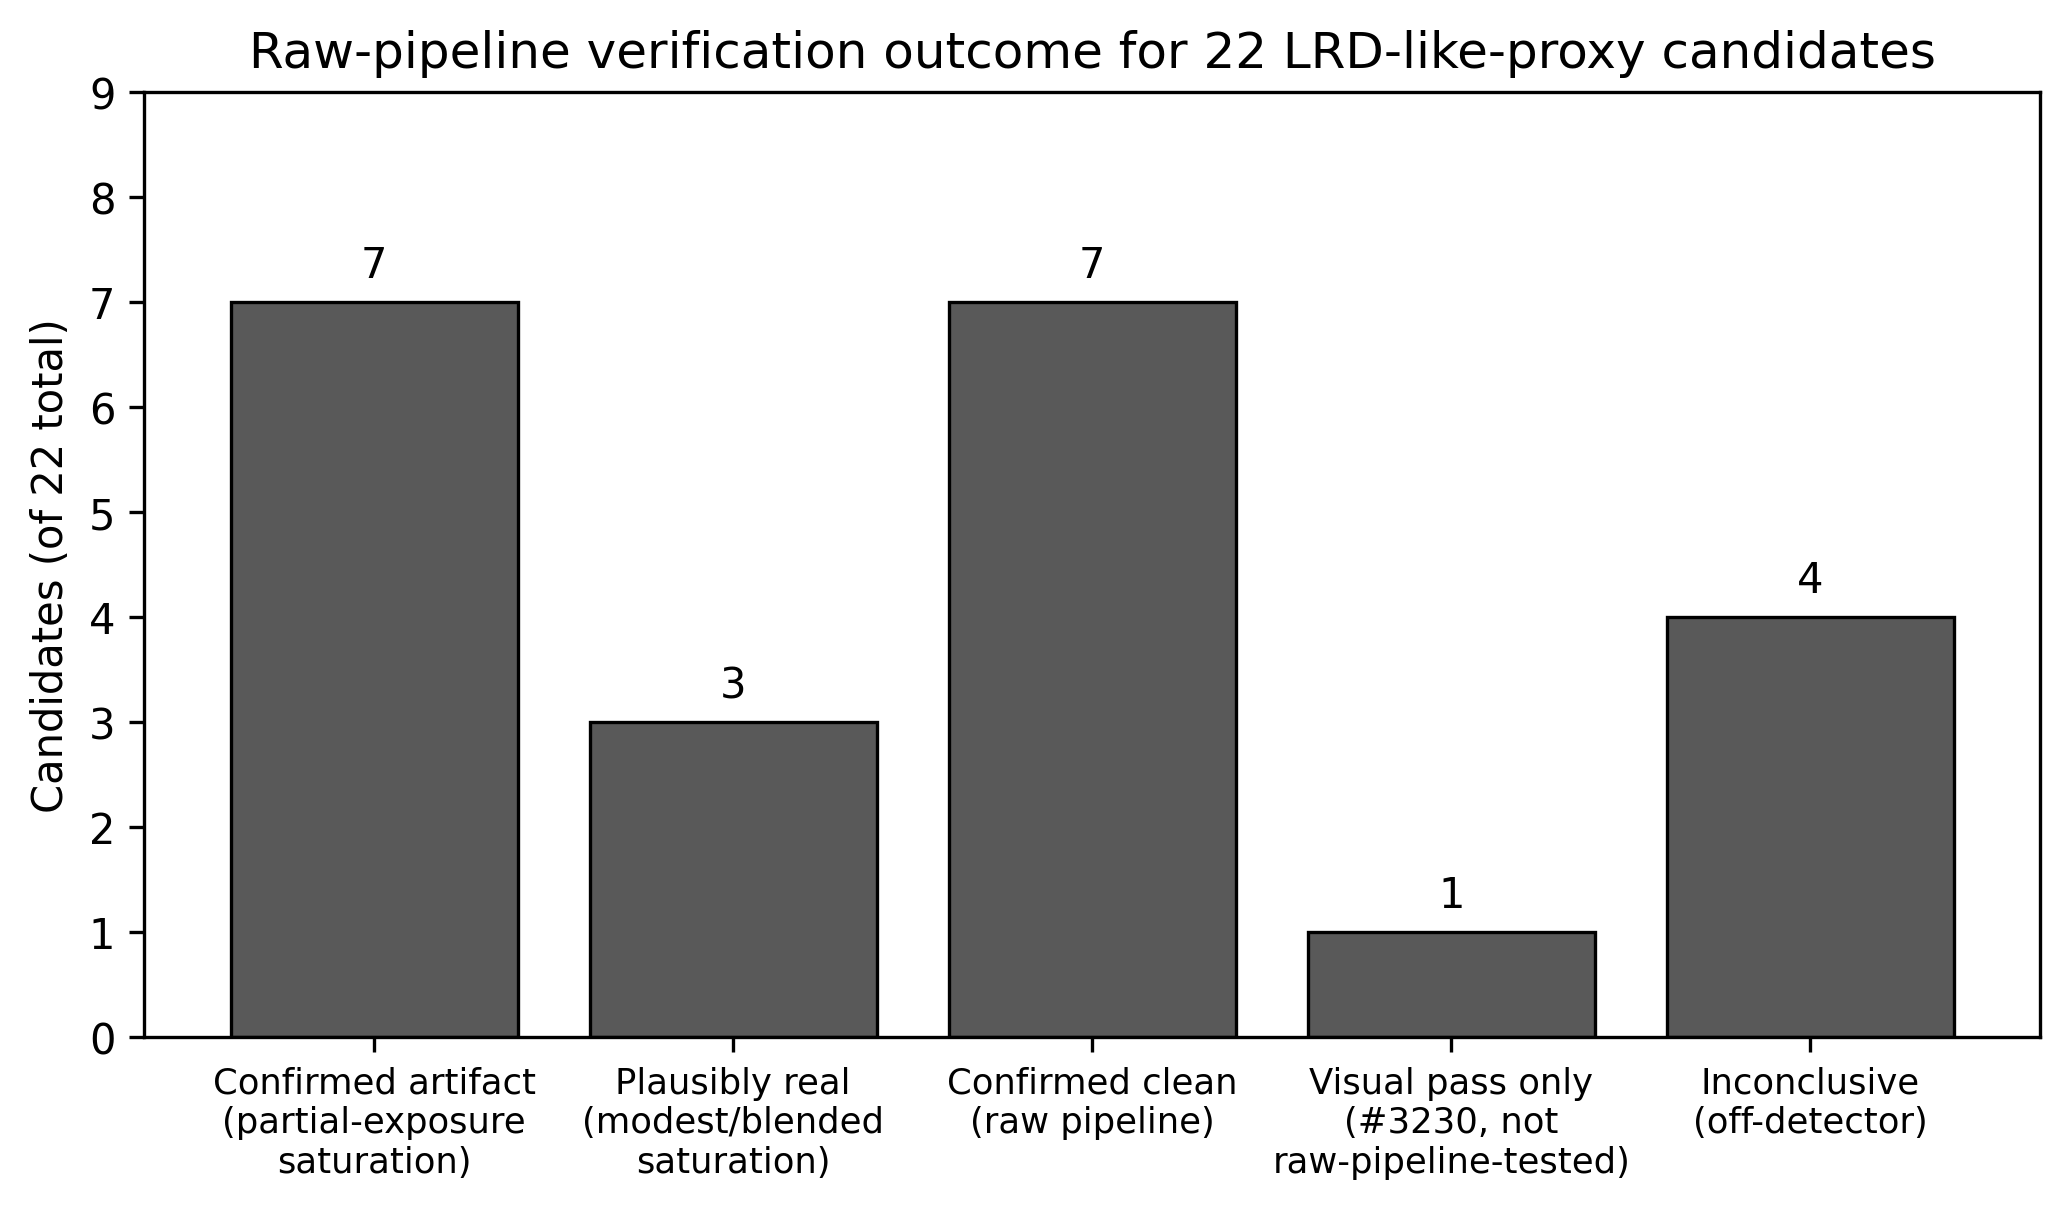
\includegraphics[width=\linewidth]{classification_summary.png}
\caption{Round 2 outcome for all 22 candidates. ``Visual pass only'' is GOODS-N
\#3230, corrected in this version of the manuscript to no longer be counted as
raw-pipeline-confirmed (Sec.~4.3).}
\label{fig:summary}
\end{figure}

The 7 confirmed artifact-consistent candidates are \#973, \#870, \#3591, \#3822,
\#4731, \#268, \#812. The 3 plausibly-real candidates (\#632, \#679, \#839) show
modest, partial saturation better explained by a genuinely bright or blended real
source than a fresh cosmic-ray hit: \#632, for instance, is independently
catalogued in SIMBAD as ZFOURGE CDFS 6130, and its two saturated exposures come
from the same visit, consistent with an ordinary bright-source peak-pixel
saturation rather than a stochastic event. The 7 confirmed-clean candidates
(\#188, \#97, \#1753, \#1206, \#450, \#1933, \#34) show zero saturation in every
exposure covering their position (Figs.~\ref{fig:cutout_97},
\ref{fig:cutout_34}). The 4 inconclusive candidates (\#4671, \#765, \#2779,
\#2300) never landed on-detector in any downloaded F444W exposure: unresolved
whether that reflects incomplete data coverage or a genuine absence, and not
counted toward either the artifact or clean tallies.

\begin{figure}[H]
\centering
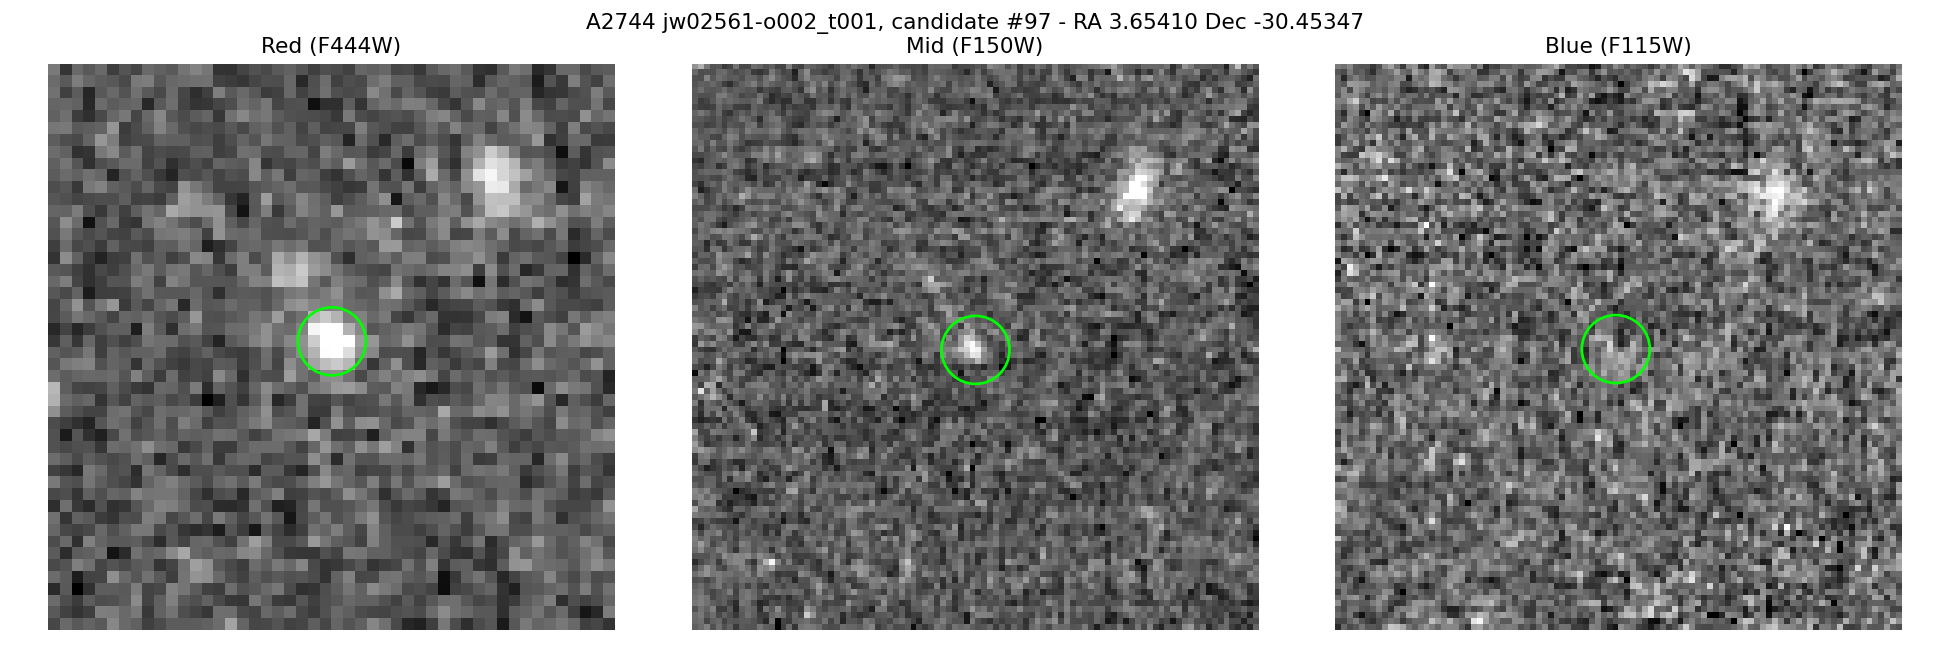
\includegraphics[width=\linewidth]{cutout_97.png}
\caption{A2744 candidate \#97, confirmed clean under the raw-pipeline test (zero
saturation in all 6 covering exposures) and already independently supported by a
dedicated EAZY photometric-redshift fit in earlier work.}
\label{fig:cutout_97}
\end{figure}

\begin{figure}[H]
\centering
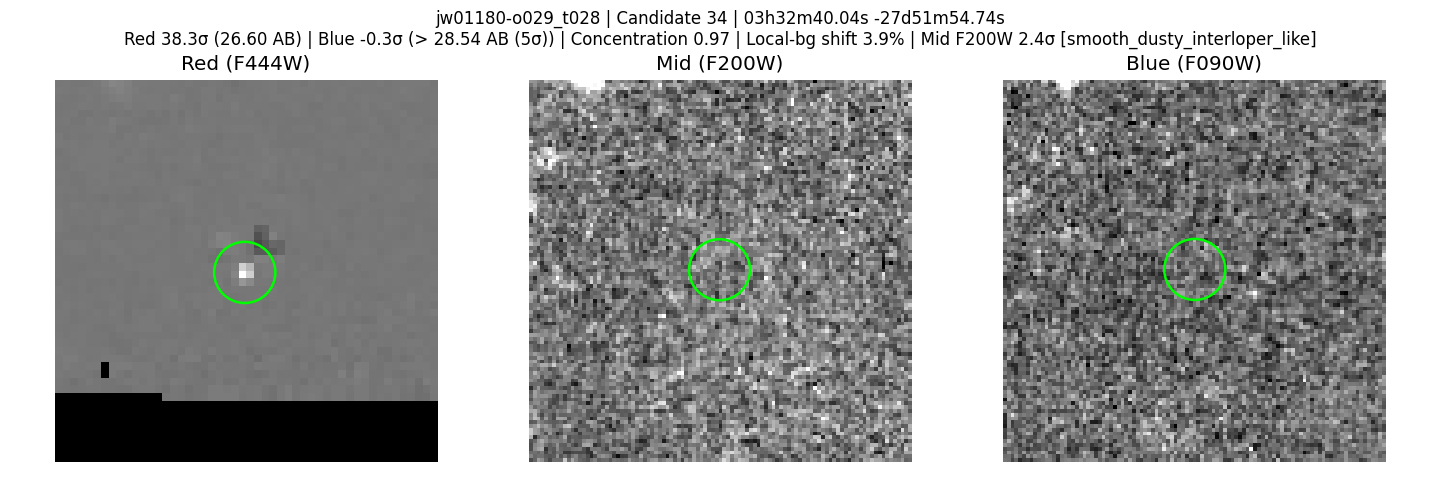
\includegraphics[width=\linewidth]{cutout_34.png}
\caption{JADES candidate \#34, confirmed clean under the raw-pipeline test and
uncatalogued, the one genuinely new, unflagged candidate this project's earlier
JADES rerun produced.}
\label{fig:cutout_34}
\end{figure}

\subsection{A correction found while preparing this manuscript}

An earlier internal working draft of this result counted GOODS-N \#3230 among the
raw-pipeline-confirmed-clean candidates, giving 8 of 22 rather than 7. Checking
that claim directly against the actual pipeline output, the candidate list
\texttt{run\_all.py} was configured with, and the \texttt{FINAL SUMMARY} block
each run produces, found \#3230 was never included in either. Its earlier
``clean'' status comes from the Round 1 visual pass alone (Table~\ref{tab:round1}
counts it there), not from a raw DQ-flag check like the other 7. We report the
correct, verified number here (7 of 22, not 8) and flag \#3230 as an open item
(Sec.~6) rather than silently absorb the discrepancy; this project's own
recurring lesson is that a working note's own summary can drift from what its
underlying data actually shows, and is only caught by checking the primary
output directly.

The visual pass and the raw-data test agreed on roughly 7 of 10 non-clean calls
checked, and disagreed on 3: \#1753, \#1206, and \#450 were called artifact-like
or ambiguous by eye but returned clean under real DQ flags. That disagreement
rate is itself informative: evidence the visual triage was tracking something
real rather than confirmation bias (it produced falsifiable predictions, and
roughly a third of them failed when checked against real data), while also
demonstrating why the raw-pipeline step was necessary rather than optional.

\section{Literature Context}

This phenomenon is field-recognized, not a new discovery. NIRCam ``snowball''
events, large cosmic-ray strikes depositing charge across up to several hundred
pixels, are a documented detector artifact class, and Stage 3's outlier-rejection
step needs redundant dithered exposures to reject them reliably. COSMOS-Web's own
reduction paper states that roughly 51\% of its survey area has only 1-2
exposures per pixel, degrading outlier rejection, without quantifying the
resulting false-positive rate for downstream source catalogs \cite{Franco2025}.
That is the literature-level version of what this project found independently in
its own data: JADES tile \texttt{o030\_t028}, with only 6 input exposures in its
F444W mosaic, is excluded by this project's own exposure-count quality gate for
exactly the same reason, before this study ever began.

\texttt{snowblind} is the field's published standard mitigation, adopted by
RUBIES and PANORAMIC specifically because LRDs' point-like appearance in red
bands makes them easy to confuse with snowball artifacts \cite{Hviding2025}. A
separate, unrelated contamination mechanism, foreground brown dwarfs, whose
near- to mid-infrared colors can mimic a reddened AGN, is also already a
quantified concern in the literature: three spectroscopically-confirmed cases in
one early sample \cite{Langeroodi2023}, and a brown-dwarf contamination fraction
as high as $\sim$25\% in one published NIRCam LRD selection, against a
$\sim$0.1\% baseline in general deep-field surveys \cite{Tu2025}. Both mechanisms,
snowball artifacts and brown-dwarf contamination, are different in kind from
this project's originally-suspected background systematic, but the same shape of
problem: photometric compact-plus-red selection alone is not sufficient, and the
field already treats this as an accepted, if incompletely quantified, risk.

\section{Extension to a Fifth Field: NEXUS (2026)}
\label{sec:nexus}

The four fields above share a common feature: all were reduced with enough dithered
exposure redundancy that, SMACS aside, the dominant contaminant found was still
detector artifacts surviving into Stage-3 mosaics, not an intrinsic limit of the
data itself. A genuinely fresh test of whether this contamination mechanism
generalizes needs a survey built from the ground up with lower redundancy. The
North Ecliptic Pole EXtragalactic Unified Survey (NEXUS), a JWST Multi-Cycle
(2024--2028) Treasury program \cite{Shen2024nexus}, provides exactly that
opportunity. Its Deep-tier public quick-release imaging uses only a two-point
dither pattern per epoch; the release documentation distributed with the data
itself states that this produces ``pixelated'' PSF shapes severe enough to
warrant an alternate, coarser-pixel-scale product specifically to mitigate it
\cite{NEXUSqdr2026}, confirmed independently here via a direct MAST query: each
released episode's F444W mosaic is built from exactly two dithered exposures per
tile-pointing, no more. This section applies the same raw-DQ persistence method
to that survey's first public Deep-tier episode (ep01, downloaded 2026-08-16),
independently of, and using none of, the four-field candidate catalogs above.

\subsection{Adapted selection and two real bugs found and fixed}

NEXUS's Deep-tier public release provides only two photometric bands (F200W,
F444W), not the three-band blue/mid/red classification used in Sec.~3; the proxy
here is a compact-plus-red-color cut instead: a \texttt{DAOStarFinder} detection
pass on the F444W mosaic, followed by a concentration cut identical to Sec.~3
($[0.65,1.00]$) and an F200W non-detection requirement ($<2\sigma$).

An initial pass at this detection, before the result below, produced clearly
unphysical significance values (up to 14866$\sigma$) traced to two real bugs in
the detection script rather than to the data: a single sigma-clipped noise
estimate for the entire mosaic, rather than the true per-pixel value from NEXUS's
own published error maps (found to be 2.6--45$\times$ higher than the flat
estimate at several spot-checked positions); and no check that a candidate's
aperture actually had real pixel coverage in the fainter band, so positions
landing in coverage gaps silently registered as spuriously ``faint and red.''
Both are fixed in the version reported here: significance is computed from the
real per-pixel error extension integrated over each aperture, and a candidate is
only kept if at least 90\% of both apertures' pixels are real, finite, non-zero
data. With both fixes applied, the maximum significance across the same mosaic
falls to 130.1$\sigma$, and the final candidate count falls from 74 to 18, in the
same range as this paper's own four fields (3--8 per field).

\subsection{Results}

None of the 18 candidates match SIMBAD or Gaia DR3 within 3$''$ (cross-checked
directly by computing angular separation from the returned coordinates, not by
trusting a query package's own convenience distance column, which returned
spurious 400+$''$ ``matches'' on a first attempt). Applying the same
persistence criterion as Sec.~4, across two independent NEXUS episodes where
multi-exposure coverage allowed it (Table~\ref{tab:nexus_results}):

\begin{table}[H]
\centering
\caption{Raw-DQ persistence test, NEXUS Deep-tier ep01, 18 candidates.}
\label{tab:nexus_results}
\begin{tabular}{lc}
\toprule
Outcome & Candidates \\
\midrule
Confirmed artifact-consistent (partial-exposure saturation) & 2 \\
Confirmed clean (zero saturation, all covering exposures) & 13 \\
Inconclusive (only 1 covering exposure available) & 1 \\
No coverage in either episode checked & 2 \\
\midrule
Total & 18 \\
\bottomrule
\end{tabular}
\end{table}

The 2 confirmed artifacts (candidates at RA/Dec 268.39450,65.18833 and
268.60903,65.22935 in this ep01 mosaic) each show \texttt{SATURATED} flags in
exactly one of several independent covering exposures spanning two separate
NEXUS episodes: one of four looks for the first, one of three for the second,
the same stochastic, epoch-specific pattern established as decisive in
Sec.~4.1. The 13 confirmed-clean candidates show zero saturation across
2--4 independent looks each.

\subsection{Interpretation}

At 2 of 18 (11\%), the confirmed contamination rate found here is real but lower
than the 32\% (7 of 22) found across the four fields in Sec.~4, and this
comparison should be treated cautiously rather than as a like-for-like survey
ranking: NEXUS's own team already documents the two-dither risk qualitatively
(without a quantified false-positive rate, the same acknowledged-but-unmeasured
gap already discussed for COSMOS-Web in Sec.~5) but never claims a specific rate;
this section's 18-candidate sample is smaller than the original 22; and most of
the confirmed-clean NEXUS candidates have only 2--4 independent exposures behind
them, fewer than several of this paper's original four-field candidates. What
this section does establish directly, rather than by analogy, is that the same
contamination mechanism and the same detection method both generalize: a
compact-plus-red photometric cut over a newly-public, low-redundancy JWST survey
released in 2026 is measurably, non-trivially contaminated by the identical
failure mode already characterized in Sec.~4, extending rather than merely
repeating this paper's original finding.

\section{Discussion}

Three points follow from this result.

\textbf{The originally-suspected mechanism was not the dominant one found.} This
study began from a specific, already-known systematic, the NIRCam module A/B
background offset corrected in \cite{Jarvis2026a}, and asked whether it distorts
LRD-like selections the same way. All candidates here were already drawn from the
current-best, source-masked-background generation of this project's catalogs, so
that specific systematic is controlled for by construction. The dominant
contaminant found instead is a different, more mundane one: transient detector
artifacts surviving into Stage-3 mosaics when exposure redundancy is low.

\textbf{Vetting status, not field identity, explains the clean/contaminated
split.} SMACS's proxy-flagged candidates are 3 for 3 clean; the other three
fields' are roughly 30-45\% clean depending on exactly how \#3230 and the
inconclusive candidates are counted. The field that came back clean is also the
only one whose candidates had already been through this project's full
multi-round vetting pipeline before this study began. That is the strongest
reading of this result: an automated compact-plus-red cut, even applied to the
current-best background-corrected catalogs, is not by itself a trustworthy
selection criterion, but the gap closes once real vetting, visual inspection at
minimum, raw-pipeline snowball-checking at best, is actually applied.

\textbf{This is an independent, if crude, quantification of an acknowledged
literature gap.} COSMOS-Web's own reduction paper states plainly that it does not
quantify a resulting false-positive rate from degraded outlier rejection
\cite{Franco2025}. The 32\% (7 of 22) confirmed-artifact rate reported here, using
real raw-exposure DQ flags rather than a visual estimate, is a genuine, if
informal and small-sample, contribution toward that open question, not proof
that any particular published LRD sample carries a comparable contamination rate,
since professional survey pipelines typically already run snowball-masking as
standard practice, which this project's ad hoc pipeline had not.

\textbf{The mechanism and the method both generalize to a new survey.} Sec.~6's
NEXUS extension was built and tested independently of the four fields above, on
data that did not exist when this study began, and still finds real (if lower,
2 of 18, 11\%) confirmed contamination via the identical persistence criterion.
The lower rate is consistent with, not in tension with, this paper's central
claim: NEXUS's own documentation already flags the same two-dither risk that
drives contamination in this paper's own fields, and the survey has not yet
published a quantified rate of its own, the same acknowledged-but-unmeasured
gap already noted for COSMOS-Web. A single-survey measurement risked being an
idiosyncrasy of this project's own four-field candidate catalogs; finding the
same failure mode, at a real if smaller rate, in an independently-built sample
from a different survey is stronger evidence that the underlying mechanism, not
this paper's own pipeline, is what drives it.

\section{Caveats and Open Threads}

This result should be read with several explicit limitations in mind.

\begin{itemize}
    \item \textbf{Small sample.} 22 candidates from four fields is not a
    statistically powered survey; the 32\% figure is a real, direct measurement
    on this specific sample, not a claim about the true LRD contamination rate in
    general.
    \item \textbf{The raw-pipeline test detects one failure mode only.} It
    specifically tests for cosmic-ray/snowball-type transient saturation. It does
    not test for pure neighbor blending (a smooth real wing adding flux with no
    DQ flag at all); the visually-flagged blend candidates in this sample are
    untested by this method and would need a different check.
    \item \textbf{Candidate \#3230's status is now understated, not overstated,
    following the correction in Sec.~4.3.} It remains visually clean and was
    never shown to be contaminated; it simply has not yet received the same
    raw-pipeline confirmation as the other 7 confirmed-clean candidates. Running
    it through the existing, already-working pipeline (its tile's raw exposures
    are already downloaded, having been used for the \#973 case study) is a
    direct, low-cost next step.
    \item \textbf{4 candidates remain genuinely unresolved} (\#4671, \#765,
    \#2779, \#2300); whether their absence from the downloaded exposures
    reflects an incomplete data pull or a real absence has not been determined.
    \item \textbf{The 7 confirmed-clean candidates were not taken further.} One,
    A2744 \#97, already has an unused EAZY photometric-redshift fit from earlier,
    unrelated work; none of the 7 have been pursued as LRD candidates in their
    own right, which was never the goal of this selection-systematics study.
    \item \textbf{The NEXUS extension (Sec.~6) uses only two photometric bands.}
    NEXUS's public Deep-tier release does not yet include a blue band suitable
    for the three-band blue/mid/red classification used in the four fields
    above; its proxy selection is compact-plus-red-color only, a weaker cut than
    the rest of this paper uses, applied because it is the best available on
    this survey's current public data, not because it is preferred.
    \item \textbf{2 of the 18 NEXUS candidates (including the single most
    significant, at 130.1$\sigma$) have no raw-exposure coverage in either of
    the two episodes checked}, and 1 has only a single covering exposure,
    insufficient for the persistence test; a third independent NEXUS episode,
    not yet checked, would be needed to resolve them.
\end{itemize}

\section{Conclusion}

An automated ``compact, smooth red continuum'' proxy for LRD-like selection,
applied to this project's own current-best NIRCam catalogs across four fields,
is contaminated at a real, measured rate: 7 of 22 flagged candidates in
previously-unvetted fields are confirmed, not merely suspected, NIRCam snowball
artifacts, using the field's own standard raw-pipeline diagnostic tool. The
originally-suspected background systematic that motivated this study was not the
dominant contaminant found; low-exposure-redundancy detector artifacts were,
consistent with (and an independent measurement toward) a gap explicitly left
open in the published literature. The clearest actionable finding is that vetting
status, not field or instrument identity, separates the one clean field from the
three contaminated ones; an automated cut over a NIRCam mosaic, without an
equivalent step, should be treated with real suspicion, a conclusion that holds
regardless of which side of the broader AGN-cocoon debate the wider LRD
population eventually falls on.

Extending the same raw-pipeline diagnostic to a fifth, independent field, the
NEXUS North Ecliptic Pole survey, with its own known low-dither-redundancy
risk factor, finds a lower but still real contamination rate of 2 of 18 (11\%)
compact, red, faint-blue candidates confirmed as transient single-epoch
artifacts by the same DQ-flag persistence test, plus 1 candidate left
genuinely inconclusive and 2 unresolved for lack of raw-exposure coverage. A
lower rate on a survey with roughly half the covering exposures per episode
of the original four fields is consistent with, not a contradiction of, the
central claim: contamination tracks vetting depth, and the method generalizes
cleanly to a survey it was not originally built for.

\section*{Acknowledgments}

This work is based on observations made with the NASA/ESA/CSA James Webb Space
Telescope. The data were obtained from the Mikulski Archive for Space Telescopes
(MAST) at the Space Telescope Science Institute. This research made use of
\texttt{astropy}, the \texttt{jwst} calibration pipeline, and \texttt{snowblind}
\cite{Davies2024snowblind}.

\appendix
\section{Computational pipeline} \label{sec:appendix}

\begin{enumerate}
    \item Apply the LRD-like proxy cut (concentration $\in[0.65,1.00]$,
    \texttt{smooth\_dusty\_interloper\_like} break shape) to each field's
    current-best, source-masked-background candidate catalog.
    \item Generate visual cutouts for any flagged candidate without one already
    on disk (\texttt{cutout\_lrdproxy\_a2744\_goodsn.py}).
    \item Round 1: eyeball each cutout against two known failure signatures
    (blocky/hard-edged detector artifact; blend against a bright extended
    neighbor).
    \item Round 2, per flagged tile: download raw \texttt{\_uncal.fits} exposures
    (both NIRCam long-wave modules); run the real \texttt{Detector1Pipeline} with
    \texttt{snowblind}'s \texttt{SnowblindStep} as a jump-detection post-hook
    (\texttt{batch\_tile.py}, \texttt{run\_all.py}).
    \item Per candidate: resolve which raw exposures actually cover its sky
    position using a real distortion-corrected WCS solution
    (\texttt{AssignWcsStep}, not the coarse pointing-only WCS Detector1 carries
    by default); extract \texttt{SATURATED}/\texttt{JUMP\_DET} DQ-flag footprints
    at the candidate position and at a same-exposure control region
    (\texttt{check\_extent.py}, \texttt{check\_flags2.py}, \texttt{
    check\_candidate.py}).
    \item Apply the persistence criterion: artifact-consistent if saturation is
    present in some but not all covering exposures; clean if present in none;
    plausibly-real if present in most/all with independent corroborating evidence
    (catalog crossmatch, blend context).
\end{enumerate}

\subsection{NEXUS-specific adaptation}

NEXUS's public Deep-tier release does not yet provide a blue-band mosaic
suitable for the three-band classification above, so Sec.~6 uses a reduced
two-band proxy instead, applied directly to the F444W/F200W Stage-3 mosaics
rather than to a pre-existing source catalog (\texttt{nexus\_lrdproxy\_search\_v2.py}):

\begin{enumerate}
    \item Detect compact sources on the F444W mosaic with \texttt{DAOStarFinder}
    against a flat, sigma-clipped detection threshold (coarse candidate
    generation only).
    \item For every detection, integrate the real per-pixel \texttt{ERROR}
    extension over a circular aperture to get a real noise estimate, rather
    than reusing the flat detection-threshold std for significance; this fixes
    a first-pass bug (Sec.~6.1) where the flat estimate was found to
    understate the true per-pixel noise by 2.6-45$\times$ at spot-checked
    positions.
    \item Require at least 90\% valid-pixel coverage in both the core and an
    outer concentration aperture, in both F444W and F200W, before trusting any
    flux or significance measurement at that position; this fixes a second
    first-pass bug where positions landing on masked/no-data gaps returned
    spuriously low F200W flux that passed the faint-blue cut for the wrong
    reason.
    \item Apply the same concentration window as the four-field study
    ($\in[0.65,1.00]$) plus a red-band significance floor and a faint-blue
    ceiling (both computed from the real, coverage-checked noise above) as the
    proxy selection.
    \item Apply the identical raw-exposure DQ-flag persistence test described
    above to each surviving candidate, using whichever of NEXUS's public
    episodes (of five total; two had usable aggregate MAST Level-3 records
    at the time of this analysis) actually cover its sky position.
\end{enumerate}

\begin{thebibliography}{9}

\bibitem{Rusakov2026}
K.~Rusakov et al., ``Little red dots as young supermassive black holes in dense ionized cocoons,'' Nature \textbf{649}, 574 (2026), arXiv:2503.16595.

\bibitem{InayoshiHo2025}
K.~Inayoshi and L.~C.~Ho, ``A Critical Evaluation of the Physical Nature of the Little Red Dots,'' arXiv:2512.03130 (2025).

\bibitem{Hviding2025}
R.~E.~Hviding et al., ``RUBIES: A spectroscopic census of little red dots: All point sources with v-shaped continua have broad lines,'' Astron.\ Astrophys.\ \textbf{702}, A57 (2025), arXiv:2506.05459.

\bibitem{Langeroodi2023}
D.~Langeroodi and J.~Hjorth, ``Little Red Dots or Brown Dwarfs? NIRSpec Discovery of Three Distant Brown Dwarfs Masquerading as NIRCam-selected Highly Reddened Active Galactic Nuclei,'' Astrophys.\ J.\ Lett.\ \textbf{957}, L27 (2023), arXiv:2308.10900.

\bibitem{Tu2025}
Z.~Tu, S.~Wang, X.~Chen, and J.~Liu, ``Three Brown Dwarfs Masquerading as High-redshift Galaxies in JWST Observations,'' Astrophys.\ J.\ \textbf{980}, 230 (2025), arXiv:2501.16648.

\bibitem{Franco2025}
M.~Franco et al., ``COSMOS-Web: Comprehensive Data Reduction for Wide-Area JWST NIRCam Imaging,'' submitted to Astrophys.\ J., arXiv:2506.03256 (2025).

\bibitem{Davies2024snowblind}
J.~Davies, \texttt{snowblind} (v0.2.1), \url{https://github.com/mpi-astronomy/snowblind} (2024).

\bibitem{Jarvis2026a}
P.~Jarvis, ``Background Systematics Versus Redshift: A Diagnostic Study of NIRCam Dropout Selection in SMACS J0723.3$-$7327 and JADES/GOODS-S,'' (2026), \url{https://github.com/ZaPpi3/background-systematics-versus-redshift}.

\bibitem{Shen2024nexus}
Y.~Shen et al., ``NEXUS: the North ecliptic pole EXtragalactic Unified Survey,'' arXiv:2408.12713 (2024).

\bibitem{NEXUSqdr2026}
NEXUS Collaboration, NEXUS Quick Data Release, \url{https://ariel.astro.illinois.edu/nexus/qdr/} (accessed 2026-08-16); see \texttt{nircam/readme.txt} for the dither-pattern and pixel-scale documentation cited here.

\end{thebibliography}

\end{document}
